\documentclass[a4latex]{article}
\usepackage[paper=a4paper,left=20mm,right=20mm,top=20mm,bottom=20mm]{geometry}
\usepackage{amsmath,amssymb,latexsym,amsfonts,url,rotating,dcolumn,ifthen,subfigure}
\usepackage{pslatex}
\usepackage{epstopdf}
\usepackage[mathscr]{eucal}
\usepackage[usenames]{color}
\usepackage[dvips]{hyperref}
\usepackage{longtable}
\usepackage[latin1]{inputenc}
%\usepackage[comma,authoryear]{natbib}
\usepackage{graphicx}
\usepackage{epsfig}
\usepackage{fancyhdr}
\usepackage{setspace}
\usepackage{geometry}
%\usepackage{pdflscape}
\setcounter{MaxMatrixCols}{10}
\setstretch{1.0}
\begin{document}
\widowpenalty=10000
\clubpenalty=10000
\raggedbottom
\addtolength{\topskip}{0pt plus 10pt}
\setcounter{totalnumber}{5}
\renewcommand{\topfraction}{0.9}
\renewcommand{\textfraction}{0.1}

%%\usepackage{endfloat}
%%\usepackage[light, first, bottomafter] {draftcopy}

%\bibpunct[:]{(}{)}{,}{a}{:}{,}

\title{Instructions for Eclipse/Threadneedle}
\author{Jacky Mallett  \\jacky@ru.is}
\date{October 2015} % delete this line to display the current date
%%% BEGIN DOCUMENT
\maketitle
\section{Pre-requisites}
Git plugin EGit, available from \url{http://www.eclipse.org/egit/} . Follow instructions to install EGit into eclipse, and then restart eclipse.
\section{Installing}
\paragraph{ Go to File/Import...} 
\par
Select Projects from Git and then Next
\begin{figure}[ht]
\centering
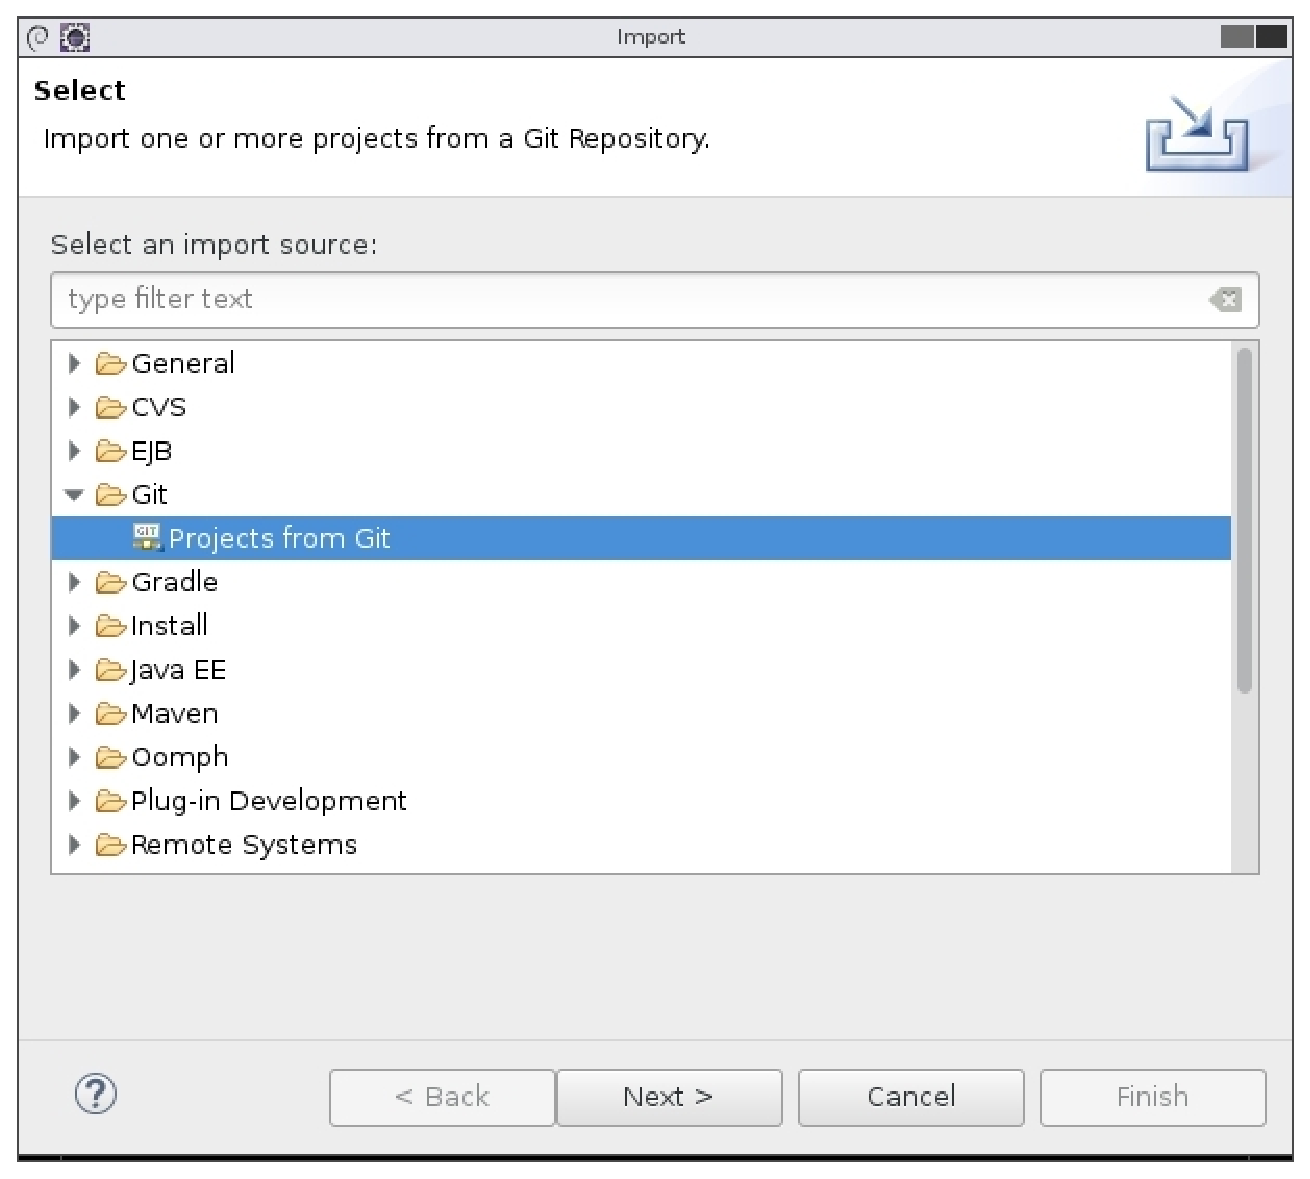
\includegraphics[height=10cm,width=10cm]{images/fig_importgit.eps}
\caption{File/Import...}
\label{fig:import}
\end{figure}

\newpage
\paragraph{Select "Clone URI"}
\begin{figure}[ht]
\centering
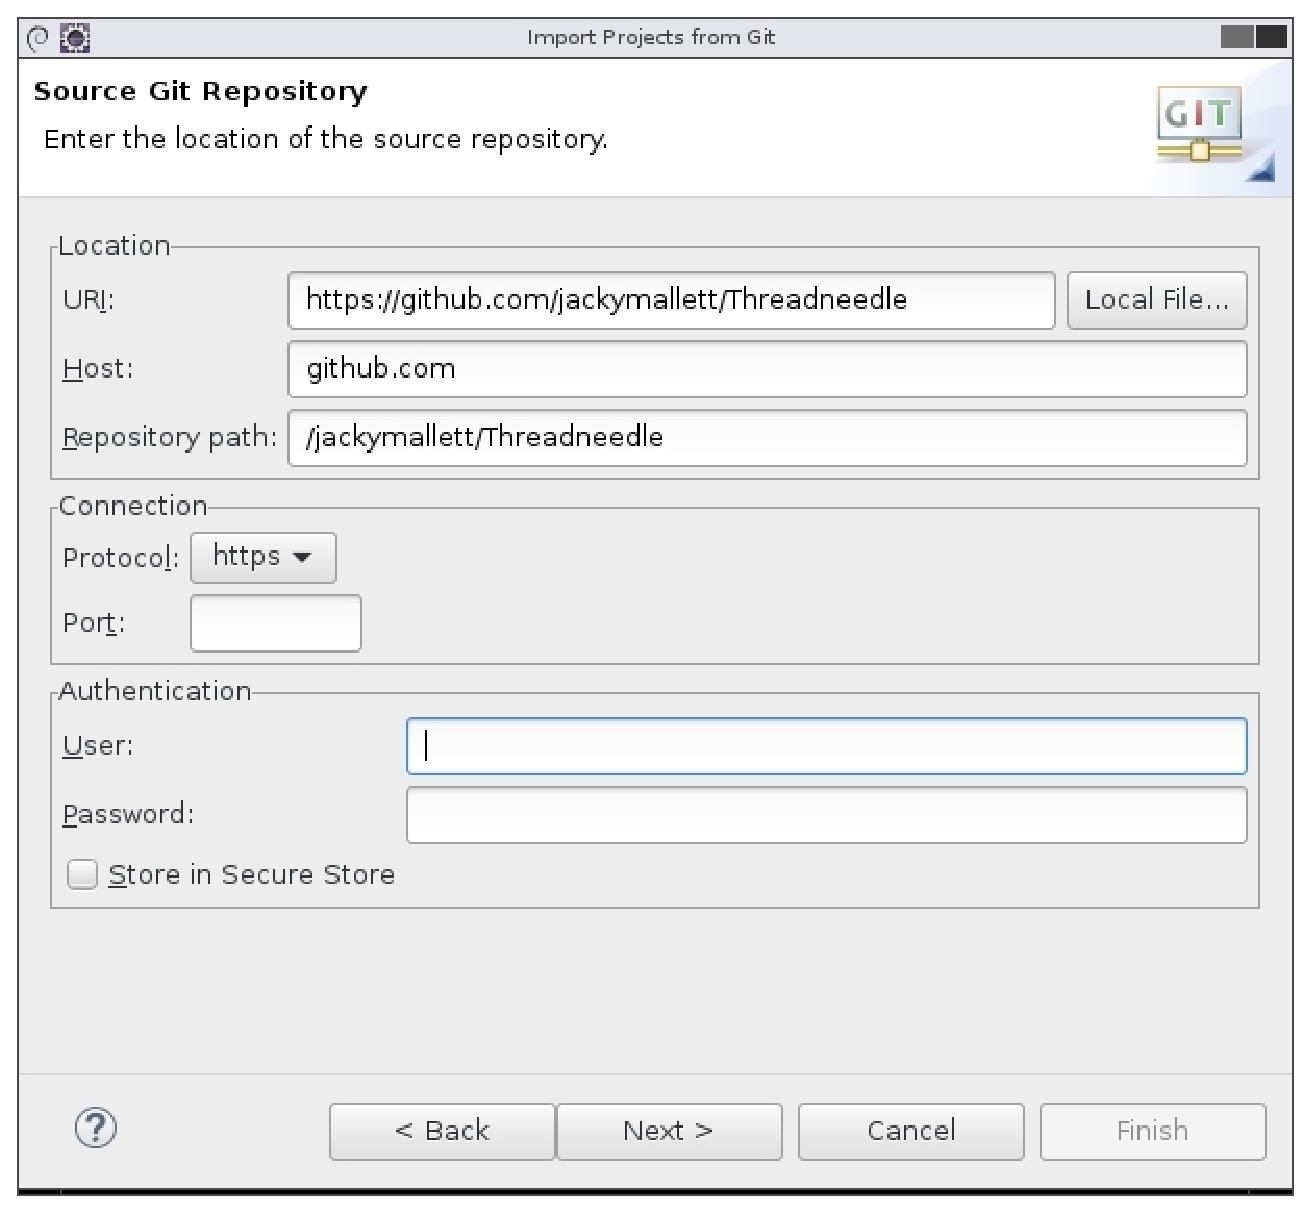
\includegraphics[height=10cm,width=10cm]{images/fig_importprojects.eps}
\caption{Import Projects from Git}
\label{fig:importprojects}
\end{figure}
\par
On the next window, enter the Threadneedle repository URI:
\begin{center}
https://github.com/jackymallett/Threadneedle
\end{center}
and your github username and password.
\newpage
\paragraph{Select Branches}
The main release branch is master.  Other branches 
can be safely ignored unless you know why you want them.
\begin{figure}[ht]
\centering
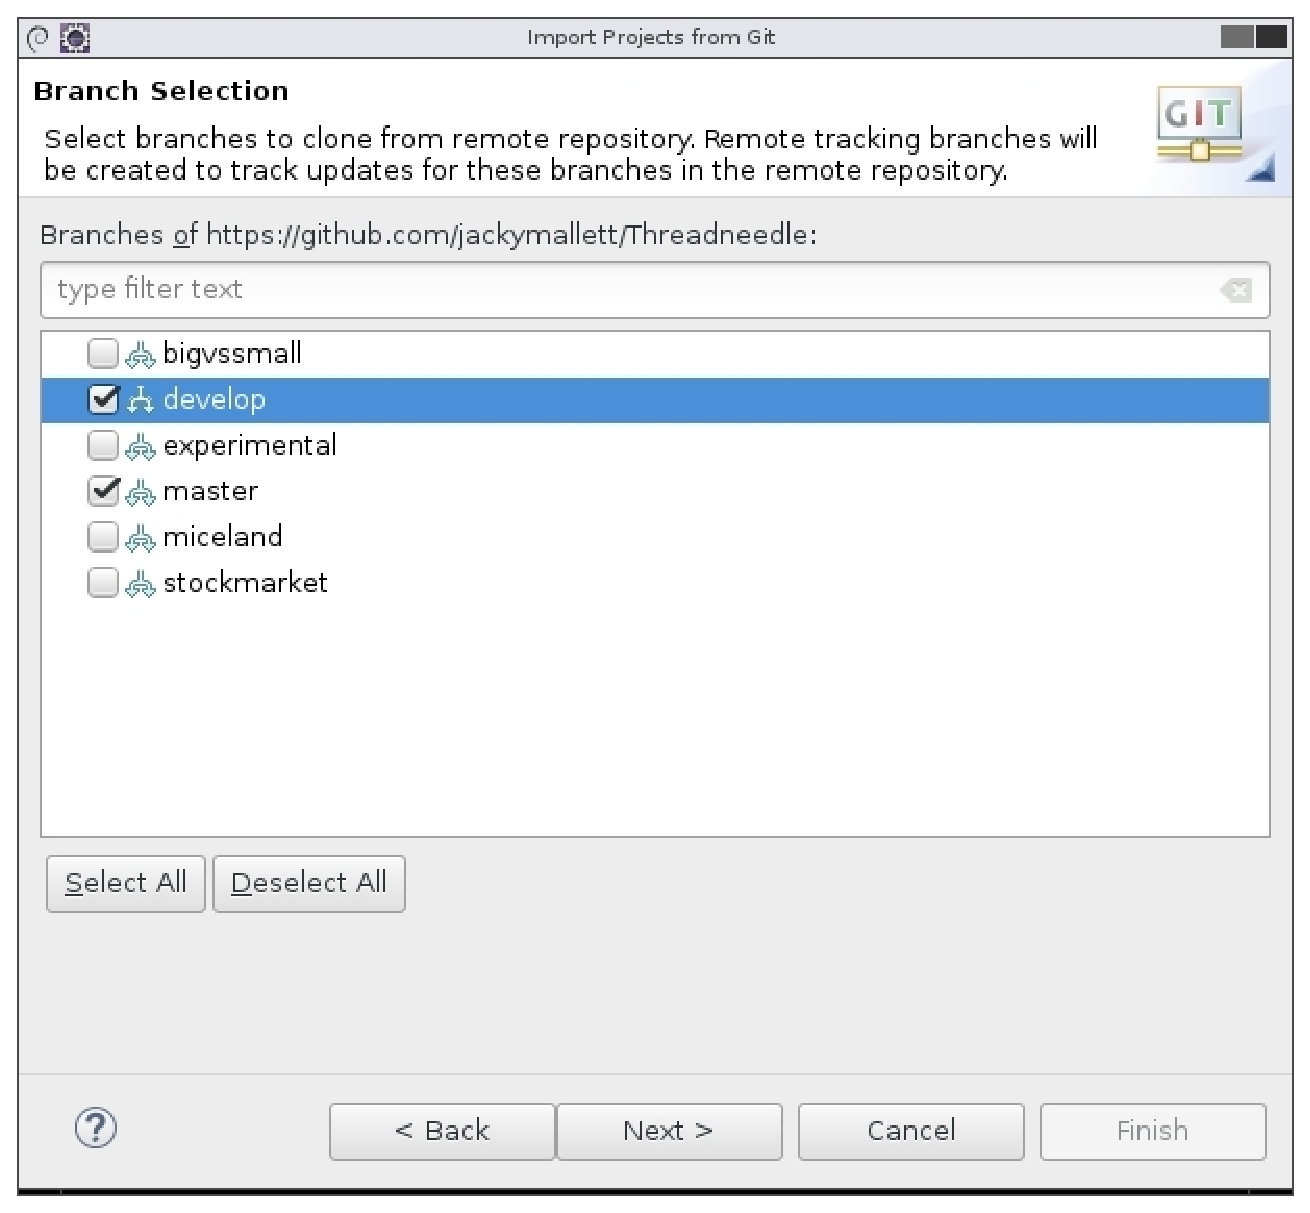
\includegraphics[height=10cm,width=10cm]{images/fig_branch.eps}
\caption{Import Projects from Git}
\label{fig:branchselection}
\end{figure}
\par
\paragraph{Set the local project directory for Threadneedle.} 
The default setting
is ~/git/Threadneedle. You may want to change this to be your eclipse
workspace directory.
\begin{figure}[ht]
\centering
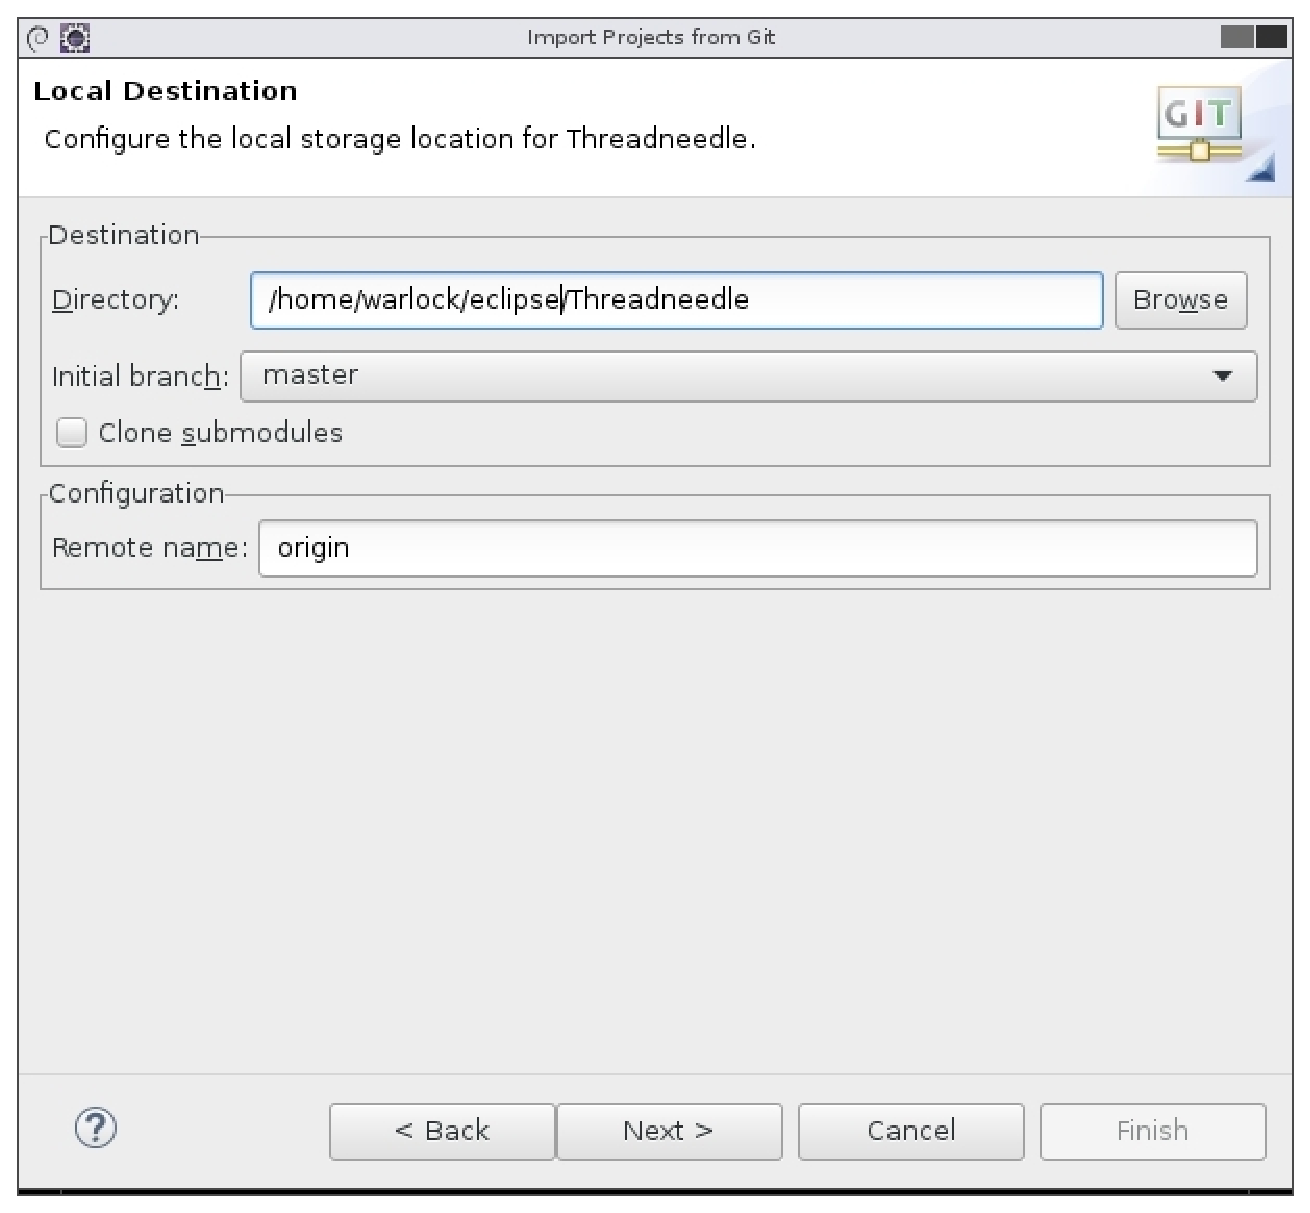
\includegraphics[height=10cm,width=10cm]{images/fig_local.eps}
\caption{Local Destination}
\label{fig:local}
\end{figure}
\par
\newpage
\paragraph{Select a wizard} 
\par
All being well, eclipse will then automatically connect to the github
repository and download it. Once that has completed, select "Import 
Using the New Project Wizard" and press Finish.
\begin{figure}[ht]
\centering
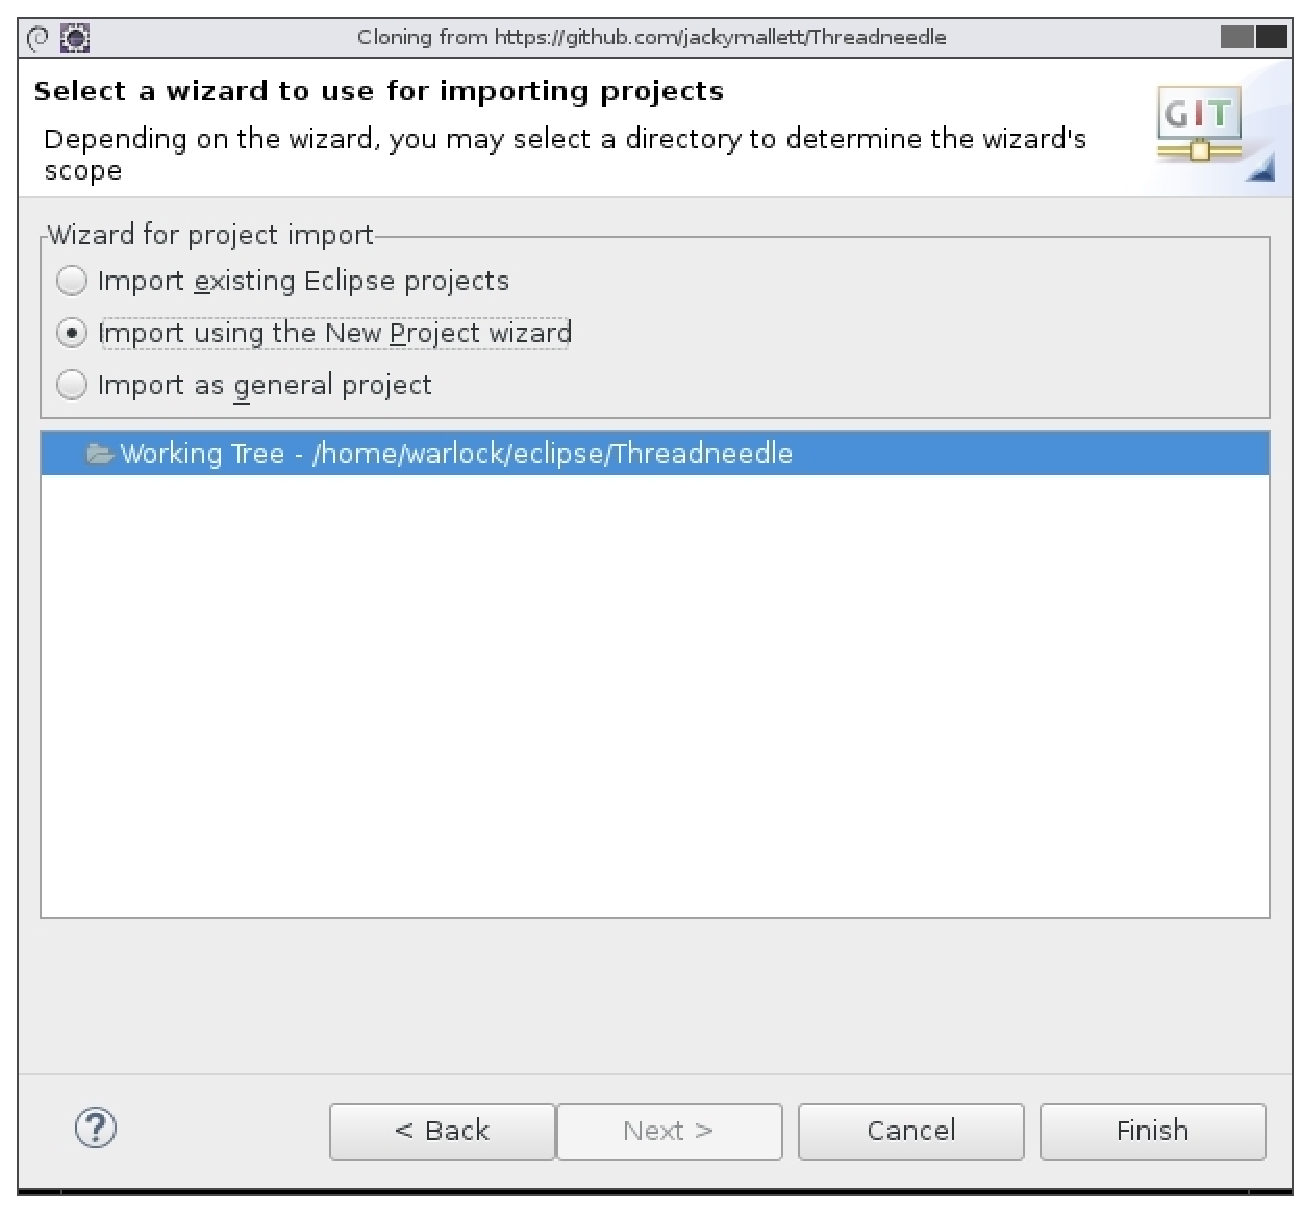
\includegraphics[height=10cm,width=10cm]{images/fig_newproject.eps}
\caption{New Project}
\label{fig:new}
\end{figure}

\paragraph{Create a Java project} 
\par
On the new "Select a wizard" screen use 
Java Project. On the next screen, put in the Project Name (Threadneedle), 
otherwise take the defaults, and select "next".
\begin{figure}[ht]
\centering
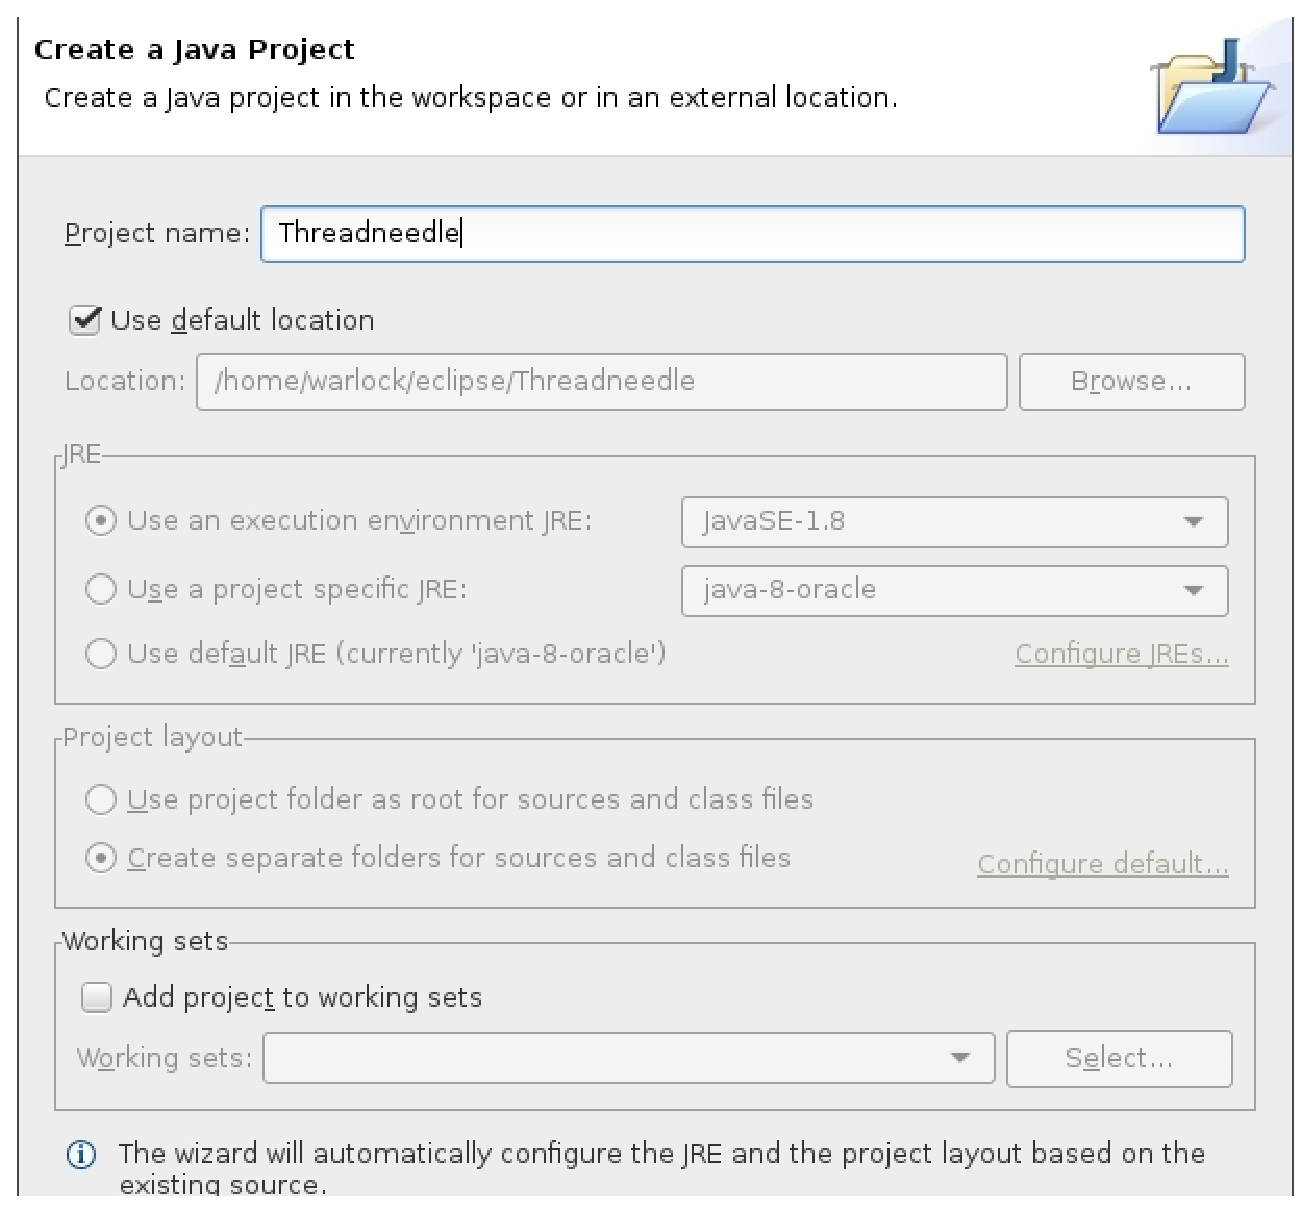
\includegraphics[height=10cm,width=10cm]{images/fig_create.eps}
\caption{Create a Java Project}
\label{fig:create}
\end{figure}
Accept the existing Java settings and press "Finish". Choose the Java
perspective that is offered.

\paragraph{Run Configuration...} 
\par
Go to the Workbench and open the Threadneedle project if necessary. 
In order to sucessfully run Threadneedle, 
you will need to tell Eclipse where to find the resources directory,
which contains the project fxml files. First, run the 
application from the IDE -  choose Java Application, and then scroll down, 
and select "Threadneedle - gui".

\begin{figure}[ht]
\centering
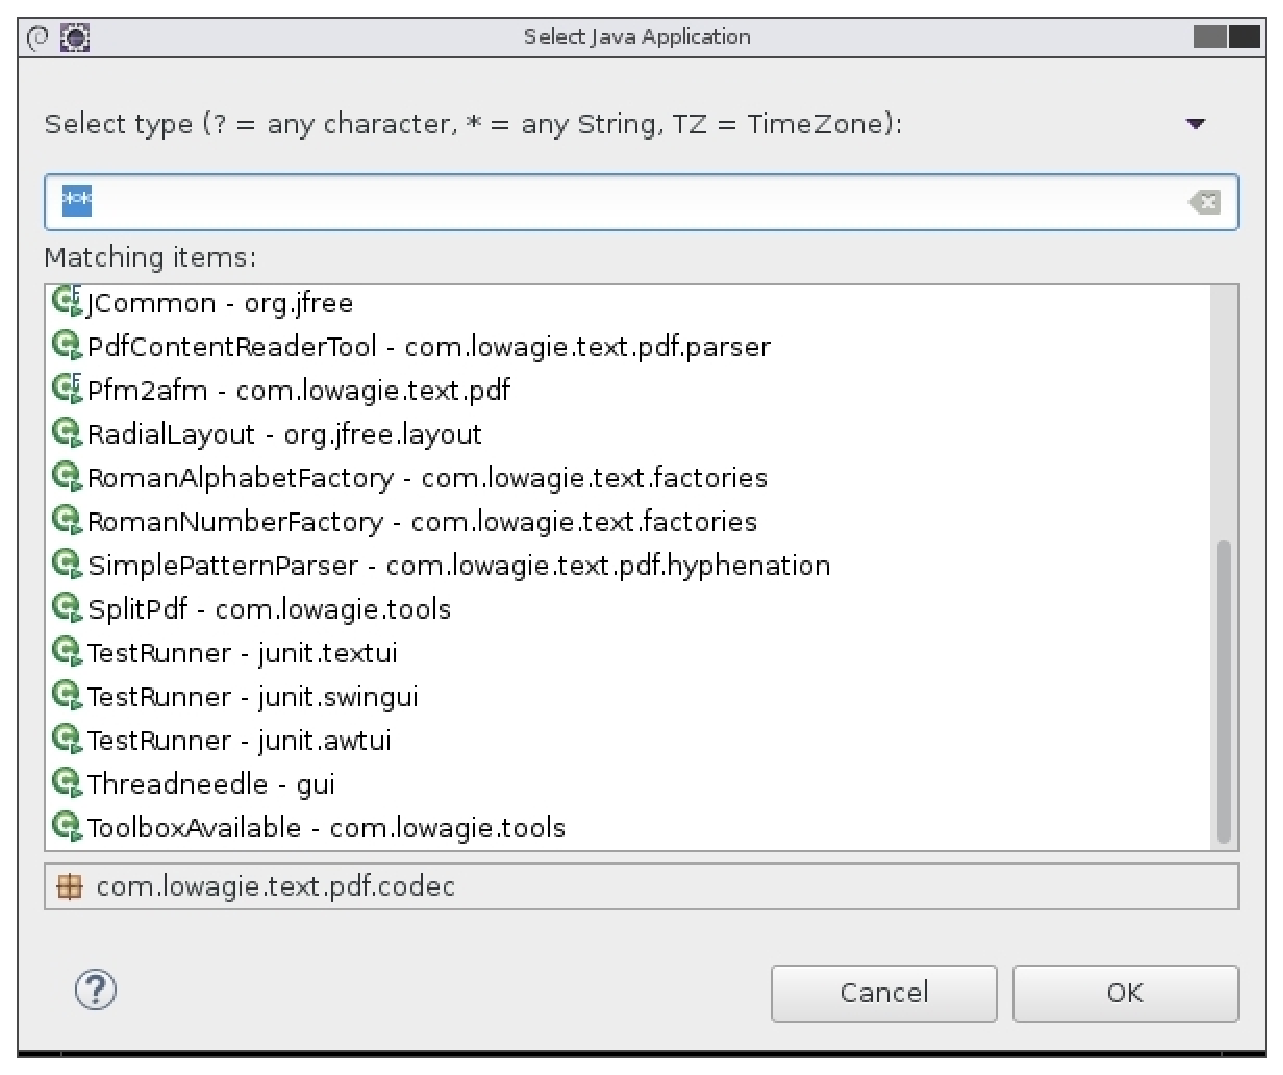
\includegraphics[height=10cm,width=10cm]{images/fig_select.eps}
\caption{Select Java Application}
\label{fig:select}
\end{figure}

This will fail, but it will add Threadneedle to the "Run Configurations".
\newpage
\paragraph{Go to Run/Run Configurations...}
Select the CLASSPATH tab. Under
"User Entries" select Advanced/Add Folder and add the directory "Threadneedle/src/resources". After applying this change, you should now be able to run 
Threadneedle from eclipse.

\begin{figure}[ht]
\centering
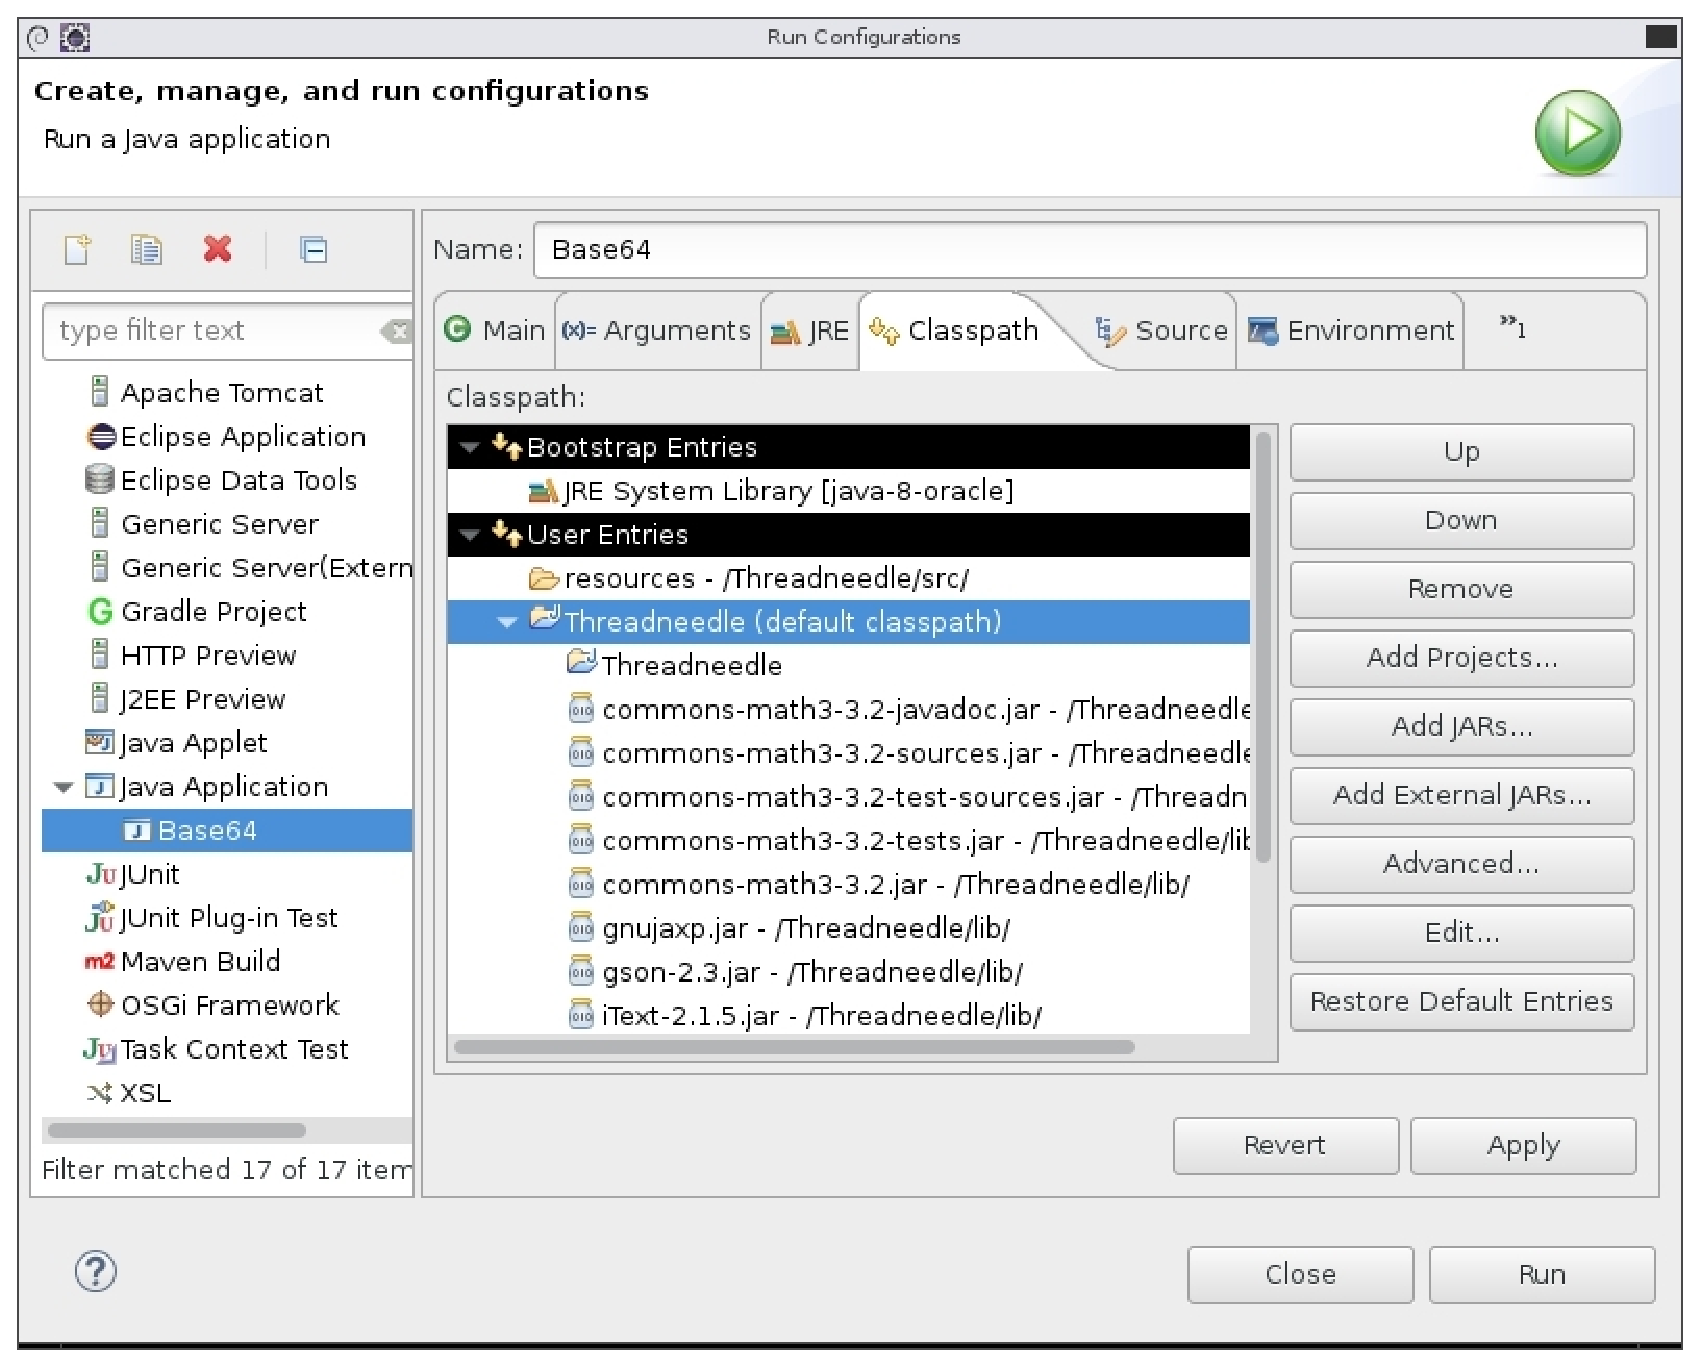
\includegraphics[height=10cm,width=10cm]{images/fig_runconfig}
\caption{Create, manage, and run configurations}
\label{fig:run}
\end{figure}

\end{document}
